\chapter{Theory}\label{chapter:theory}

\section{Ball Screw Drive}
As shown in fig. \ref{fig:Ball_Screw}, ball screw drives (BSDs) consist of steel balls, a screw shaft and nut, seals and a tube. The steel balls serve as ball bearing between the screw shaft and nut \cite{Lee2015}. The screw shaft is mounted by a fixed and free bearing and actuated by a motor \cite{DENG2020}. The screw nut, which carries the load, moves linearly along the screw shaft, which is rotated by the motor \cite{Lee2015}. Linear guiding shoes (LGSs) are installed to direct the components, which are moved linearly by the BSD \cite{DENG2020}. While the steel balls are rotated under external load and friction, the ball screw drive shaft is under constant compressive stress. Due to the rolling friction, defects usually occur in the grooves of the screw shaft, which guide the steel balls. Defects usually start with little abrasion on the surface. Each time the steel balls pass the surface defects, the system repetitively takes shocks. Depending on the location and severity of the defects the periodicity as well as the intensity of the shock varies. For this reason, vibration signals are promising to contain expressive information about the machine health condition \cite{Lee2015}. Besides that, the surface defects also lower the efficiency of the system. In order to move the load with the same speed and acceleration, the motor torque needs to be increased. Analysing the motor torque and current signals is therefore also interesting in the PHM context. Such signals can be retrieved from the machine controller \cite{AZAMFAR2020103932}.

\begin{figure}[H]
  \centering
  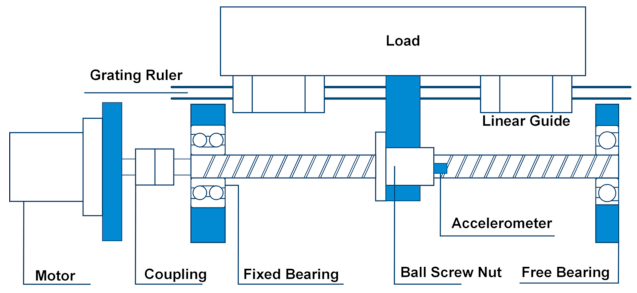
\includegraphics[width=1\textwidth]{Ball_Screw.pdf}
  \caption {Ball screw drive \cite{DENG2020}} \label{fig:Ball_Screw}
\end{figure}

\section{Neural Network}
The big data ecosystem is constantly evolving and new technologies are coming up constantly. Many of them do react more and more to the demands of the industry. Big data refers to an increase of unstructured data, high sampling rates and a variety of different data sources \cite{Sagiroglu2013}. Machine learning tries to solve data-related problems by learning to extract expressive and informative features from the data. Deep learning is a specific branch of machine learning, which is inspired by the function of human brains \cite{Calin2020}. The increased amount of data and computational power makes deep learning applications more attractive for the real-world use. Neural networks are hierarchically structured non-linear processing layers, which try to learn representations of data in different abstraction layers \cite{ZHAO2019213}. In the following, different aspects of deep learning are explained in more detail.

\subsection{Neural Network Architecture}
Neural networks consist of neurons, which are layered in a hierarchical architecture. The neurons of consecutive layers are connected through weights and biases. During the model optimization, the weights and biases are updated \cite{ShilohPerl2020}. Fig. \ref{fig:neural_network_overview} shows the organization of neurons in a fully-connected network architecture. Each neuron from layer i is connected with all neurons from layer i+1 and shares information with them.

\begin{figure}[H]
  \centering
  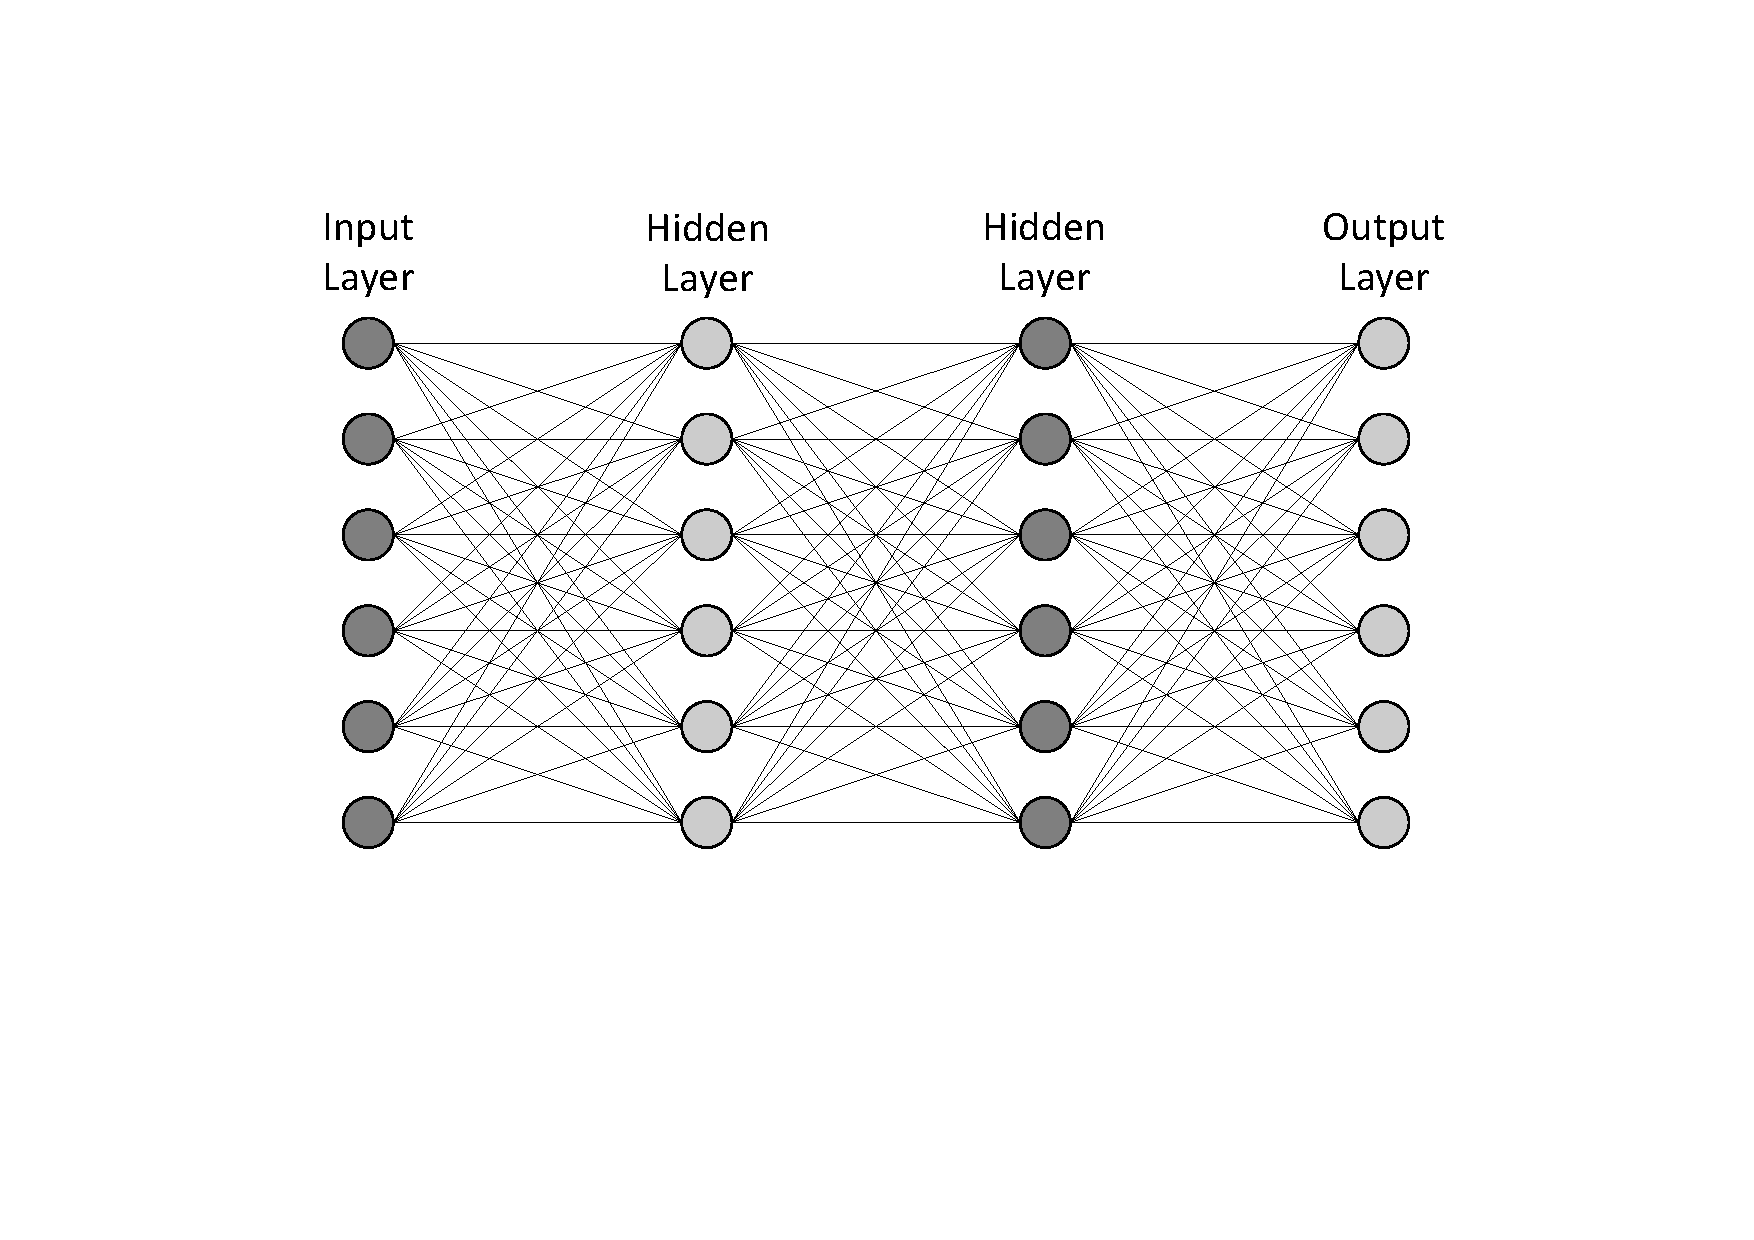
\includegraphics[width=0.7\textwidth]{neural_network_overview.pdf}
  \caption {Layer overview neural network}
  \label{fig:neural_network_overview}
\end{figure}
The input of a neuron is calculated in two steps. Firstly, the weighted sum of all previous neurons and a bias is estimated. Afterwards, an activation function is applied to the results, which gives the neural network a non-linear property \cite{ShilohPerl2020}. Standard multilayer feedforward networks with even one single hidden layer and an arbitrary bounded and non-constant activation function are universal approximators. This means that neural networks can learn to represent a wide variety of functions. When providing a sufficient number of layers and corresponding activation functions, any continuous function can be modeled arbitrarily well \cite{HORNIK1991}. Without activation functions, neural networks could only make linear assignments between inputs and outputs. Such neural networks cannot mathematically realize complex relationships in the data \cite{Ding2018}.

\subsection{Activation Function}
Activation function choices in neural networks mainly depend on the specific layer type and task to be solved. In classification tasks, one typically uses tanh, sigmoid and ReLU activations in hidden layers and a sigmoid or softmax function in the final layer \cite{ShilohPerl2020}. The sigmoid function is used for binary and the softmax for multi-class classification. The softmax function is an extension of the sigmoid function for the multi-class case. The softmax and sigmoid functions normalize the network output to a probability distribution over the predefined classes \cite{ShilohPerl2020}. Deciding for activation functions in the hidden layers does not follow such clear rules. All the mentioned functions have different characteristics, which lead to individual advantages and disadvantages. The sigmoid activation function squeezes the inputs in values between 0 and 1 and the tanh activation function between -1 and 1. Both functions can suffer from vanishing gradients, since the derivative of these functions is close to zero for very big or small inputs \cite{Calin2020}. The ReLU activation function solves that problem but maps all negative inputs to zero. This so-called dead ReLU problem is solved by the Leaky Relu functions \cite{Dubey2019}. In table \ref{tab:activation_functions} some of the most popular activation functions are described.

\begin {table}[H]
\begin{tabular}{ c c c c }
\toprule 
Formula & Formulation s(x) & Derivative $\frac{ds(x)}{dx}$ & Function Output Range \\
\midrule 
ReLU &   $\begin{cases} 0 & \text{, for }x < 0\\
	x & \text{, for }x \geqslant 0 \end{cases}$ & $\begin{cases} 0 & \text{, for }1 < 0\\
	1 & \text{, for }x \geqslant 0 \end{cases}$ & $[ 0, \infty)$\\

\rule{0pt}{5ex}%  EXTRA vertical height 

Leaky ReLU &   $\begin{cases} \alpha x & \text{, for }x < 0\\
	x & \text{, for }x \geqslant 0 \end{cases}$ & $\begin{cases} \alpha & \text{, for }1 < 0\\
	1 & \text{, for }x \geqslant 0 \end{cases}$ & $(- \infty, \infty)$\\

\rule{0pt}{5ex}%  EXTRA vertical height 

Sigmoid & $\frac{1}{1+e^{-x}}$ & $\frac{e^{-x}}{(1+e^{-x})^{2}}$ & (0,1)\\

\rule{0pt}{5ex}%  EXTRA vertical height 

Softmax & $\frac{e^{x_{i}}}{\sum_{j=1}^{K} e^{x_{j}}}$ & $\frac{e^{-x}}{(1+e^{-x})^{2}}$ & (0,1)\\

\rule{0pt}{5ex}%  EXTRA vertical height 

tanh & $\frac{e^{2x}-1}{e^{2x}+1}$ & $1-tanh^{2}(x)$ & $(-1,1)$ \\
\bottomrule  

\end{tabular}
\caption {Overview activation functions \cite{ShilohPerl2020}} \label{tab:activation_functions}
\end {table}


\subsection{Loss Function}
The loss function acts as an evaluation criterion for the neural network. During the optimization the model is adapted to decrease the loss function. Deep learning can be applied in two different use cases: (1) regression tasks and (2) classification tasks. In a regression problem, the goal is to learn a mapping function from input variables to a continuous output variable. Contrariwise, in a classification problem, the model aims to predict a class label for each input sample \cite{ShilohPerl2020}. Typically, the mean square error (MSE) is applied as criterion in regression tasks:

\begin{equation}
L(X) =  \sum_{i=0}^{N}(\hat{y}(x_{i})-y(x_{i}))^2,
\end{equation}

where $N$ is the number of training samples, $y(x_{i})$ the ground truth and $\hat{y}(x_{i})$ the predicted class label for the sample $x_{i}$ \cite{Calin2020}. On the other hand, a Cross-Entropy-loss (CE-loss) is common for classification tasks: 

\begin{equation}
L(X) = \sum_{i=0}^{N} \sum_{j=0}^{C} y_{j}(x_{i}) log(p_{j}(x_{i})),
\end{equation}
where $C$ is the number of predefined classes, $p_{j}(x_{i})$ the predicted probability of the sample $x_{i}$ belonging to the class $j$ and $y_{j}(x_{i})$ is the j-th entry of the one-hot encoding vector, representing the ground truth label of the sample $x_{i}$ \cite{ShilohPerl2020}.



\subsection{Optimizer}
The optimizer is responsible for adapting the model according to the loss function. Usually, first-order methods are used to optimize neural networks. These methods solely rely on the first-order gradients to update the model parameters. Second-order methods combine first- and second-order derivatives, which generally makes the optimization converge faster. This method requires the Hessian, whose calculation is expansive for big datasets and models \cite{Calin2020}\cite{ShilohPerl2020}. When the dataset is big, full batch gradient descent methods, which calculate the gradient from the whole dataset and update the model accordingly, suffer from long training times. The stochastic gradient descent (SGD) optimization tries to circumnavigate this problem. Repetitively, the model is updated with gradients calculated from a single sample, which is picked randomly from the dataset. Since the choice of these samples is random, the optimization suffers from instability and fluctuation \cite{ShilohPerl2020}. Therefore, a common practice is to separate the dataset in several subsets, so called mini-batches. For each mini-batch, the gradients are calculated and the model is updated accordingly. This process is repeated for all mini-batches retrieved from the dataset. A traing loop through the whole dataset is called an epoch. As soon as the loss converges, the training is terminated \cite{ShilohPerl2020}. Despite convergence, an optimal solution is not assured due to the non-convexity of neural network optimizations \cite{ShilohPerl2020}.

\subsubsection{Momentum}
In order to accelerate and stabilize the optimization, historical gradients can be included. The model parameters are updated by a moving average over the past gradients. Methods which use momentum, accelerate the optimization in the relevant directions and dampen oscillations. This gradient descent variant is able to adapt the step size in the different latent feature space dimensions. The step size is increased in the relevant and decreased in the irrelevant directions \cite{Ruder2016}. In a first step, the moving average over the past gradients is calculated and in a second step the model parameters are updated accordingly:

    \begin{equation}
      \begin{aligned}
          v_{t} = & \gamma v_{t-1} +  \eta \nabla_{\theta}L(W_{t-1}) &\\
          W_{t} = &W_{t-1} - v_{t},
          \label{eqn:momentum}
      \end{aligned}
    \end{equation}

    where $v_{t}$ is the updated and $v_{t-1}$ the current momentum, $W_{t}$ is the updated and $W_{t-1}$ the current model weights, $\nabla_{\theta}L(W_{t-1})$ is the derivative of the loss with respect to the current model weights, $\eta$ is the learning rate and $\gamma$ defines the relationship between the current momentum and gradient for calculating the updated momentum \cite{Ruder2016}.

    
\subsubsection{Nesterov Accelerated Gradient}
Another well known optimizer of this kind is the Nesterov Accelerated Gradient (NAG), which extends the regular first-order momentum update rules. When calculating the first-order momentum, NAG calculates the gradient with respect to the pre-updated weights: 

\begin{equation}
    \nabla_{\theta}L( W_{t-1} - \gamma v_{t-1}),
\end{equation}
    
where $W_{t-1}$ are the current model weights, which are pre-updated with the current first-order momentum $v_{t-1}$. This special gradient estimation is used to calculate the momentum, which is then used to update the model parameters just as described in \ref{eqn:momentum} \cite{Ruder2016}.

\subsubsection{Adagrad}
Adagrad uses a squared version of the moving average over the past gradients:

\begin{equation}
    \begin{aligned}
    W_{t} = W_{t-1} - \frac{\eta}{\sqrt{G_{t}+ \epsilon}} \bigodot \nabla_{\theta}L(W_{t-1}),
    \end{aligned}
    \label{eq:Adagrad}
\end{equation}
    
where  $W_{t-1}$ are the current and $W_{t}$ the updated model weights, $\nabla_{\theta}L(W_{t})$ is the derivative of the loss with respect to the current model weights, $G_{t}$ is the second-order momentum, which is a diagonal matrix with each diagonal element i,i being the sum of the squared first-order gradients with respect to the model parameter i, $\epsilon$ denotes a small quantity, which prevents the division by zero and $\gamma$ is the learning rate \cite{Ruder2016}.


\subsubsection{Adaptive Moment Estimation}
Adaptive Moment Estimation (Adam) is one of the most popular optimizer. ADAM combines the idea of first and second-order momentum: 
\begin{equation}
    \begin{aligned}
    &m_{t} =  \beta_{1} m_{t-1} +  (1-\beta_{1}) \nabla_{\theta}L(W_{t-1}) &\\
    &v_{t} =  \beta_{2} v_{t-1} +  (1-\beta_{2}) \nabla_{\theta}L^{2}(W_{t-1}) &\\
    &\hat{m}_{t} = \frac{m_{t}}{1-\beta_{1}^{t}}&\\
    &\hat{v}_{t} = \frac{v_{t}}{1-\beta_{2}^{t}}&\\
    & W_{t} = W_{t-1} - \frac{\eta}{\sqrt[2]{\hat{v}_{t} + \epsilon}}\hat{m}_{t}, &\\
    \end{aligned}
    \label{eq:ADAM}
\end{equation}
    
where $m_{t}$ and $v_{t}$ are the first- and second-order momentum, $\hat{m}_{t}$ and $\hat{v}_{t}$ are the bias-corrected first- and second-order momentum, $\beta_{1}$ and $\beta_{2}$ are the weighting factors for the moving average and $W_{t-1}$ and  $W_{t}$ are the current and updated model weights \cite{Ruder2016}.

\subsection{Training Loop}
During the training, the model parameters are adapted such that the loss function is minimized. In a two-stage process the model is optimized by alternately applying the forward and backward pass. At the example of a single neuron, fig. \ref{fig:neural_network_optimization} shows this optimization process in detail: 
\begin{itemize}
    \item \textbf{Forward pass}: The $i$ inputs, which are connected with the single neuron $j$ are multiplied with its weights $w_{i,j}$ and summed up together with a bias $b_{j}$. The resulting logit $z_{j}$ is then processed by the activation function $\phi$. Generally, different activation functions can be used throughout the network. After calculating the values for all neurons in the consecutive hidden layers, a loss function evaluates the prediction of the neural network \cite{AN201942}.
    \item \textbf{Backward pass}: 
    The partial derivatives of the model layers are calculated. The derivatives of the loss with respect to the weights and biases is calculated by concatenating the corresponding partial derivatives in the reverse order of the forward pass. The chain rule is used for that concatenation \cite{ShilohPerl2020}. The model parameters are updated in the negative direction of the corresponding gradient with a step size defined by the learning rate:
    \begin{equation}
        \theta = \theta - \eta \cdot {\nabla}_{\theta}J(\theta),
    \end{equation}
    where $\theta$ are the model parameters, $\eta$ is the learning rate and ${\nabla}_{\theta}J(\theta)$ the derivative of the loss function with respect to the model parameters \cite{Lydia2019}. Exemplary, the update of a the weight $w_{i,j}$ between input $i$ and the single neuron $j$ is defined as following:
    \begin{equation}
     \frac{\delta L}{\delta w_{i,j}} = \frac{\delta L}{\delta \hat{y}_{j}} \cdot \frac{\delta \hat{y}_{j}}{\delta z_{j}} \cdot \frac{\delta z_{j}}{\delta w_{i,j}}, 
     \label{chain_rule}
    \end{equation}
where $\frac{\delta L}{\delta \hat{y}_{j}}$ is the derivative of the loss $L$ with respect to the model's predicted probability of the training sample belonging to class $j$, $\frac{\delta \hat{y}_{j}}{\delta z_{j}}$ is the derivative of the activation function in the last layer, $ \frac{\delta z_{j}}{\delta w_{i,j}}$ is the derivative of the logit $z_{j}$ with respect to the weight of interest $w_{i,j}$ \cite{ShilohPerl2020}. 
\end{itemize}
\begin{figure}[H]
  \centering
  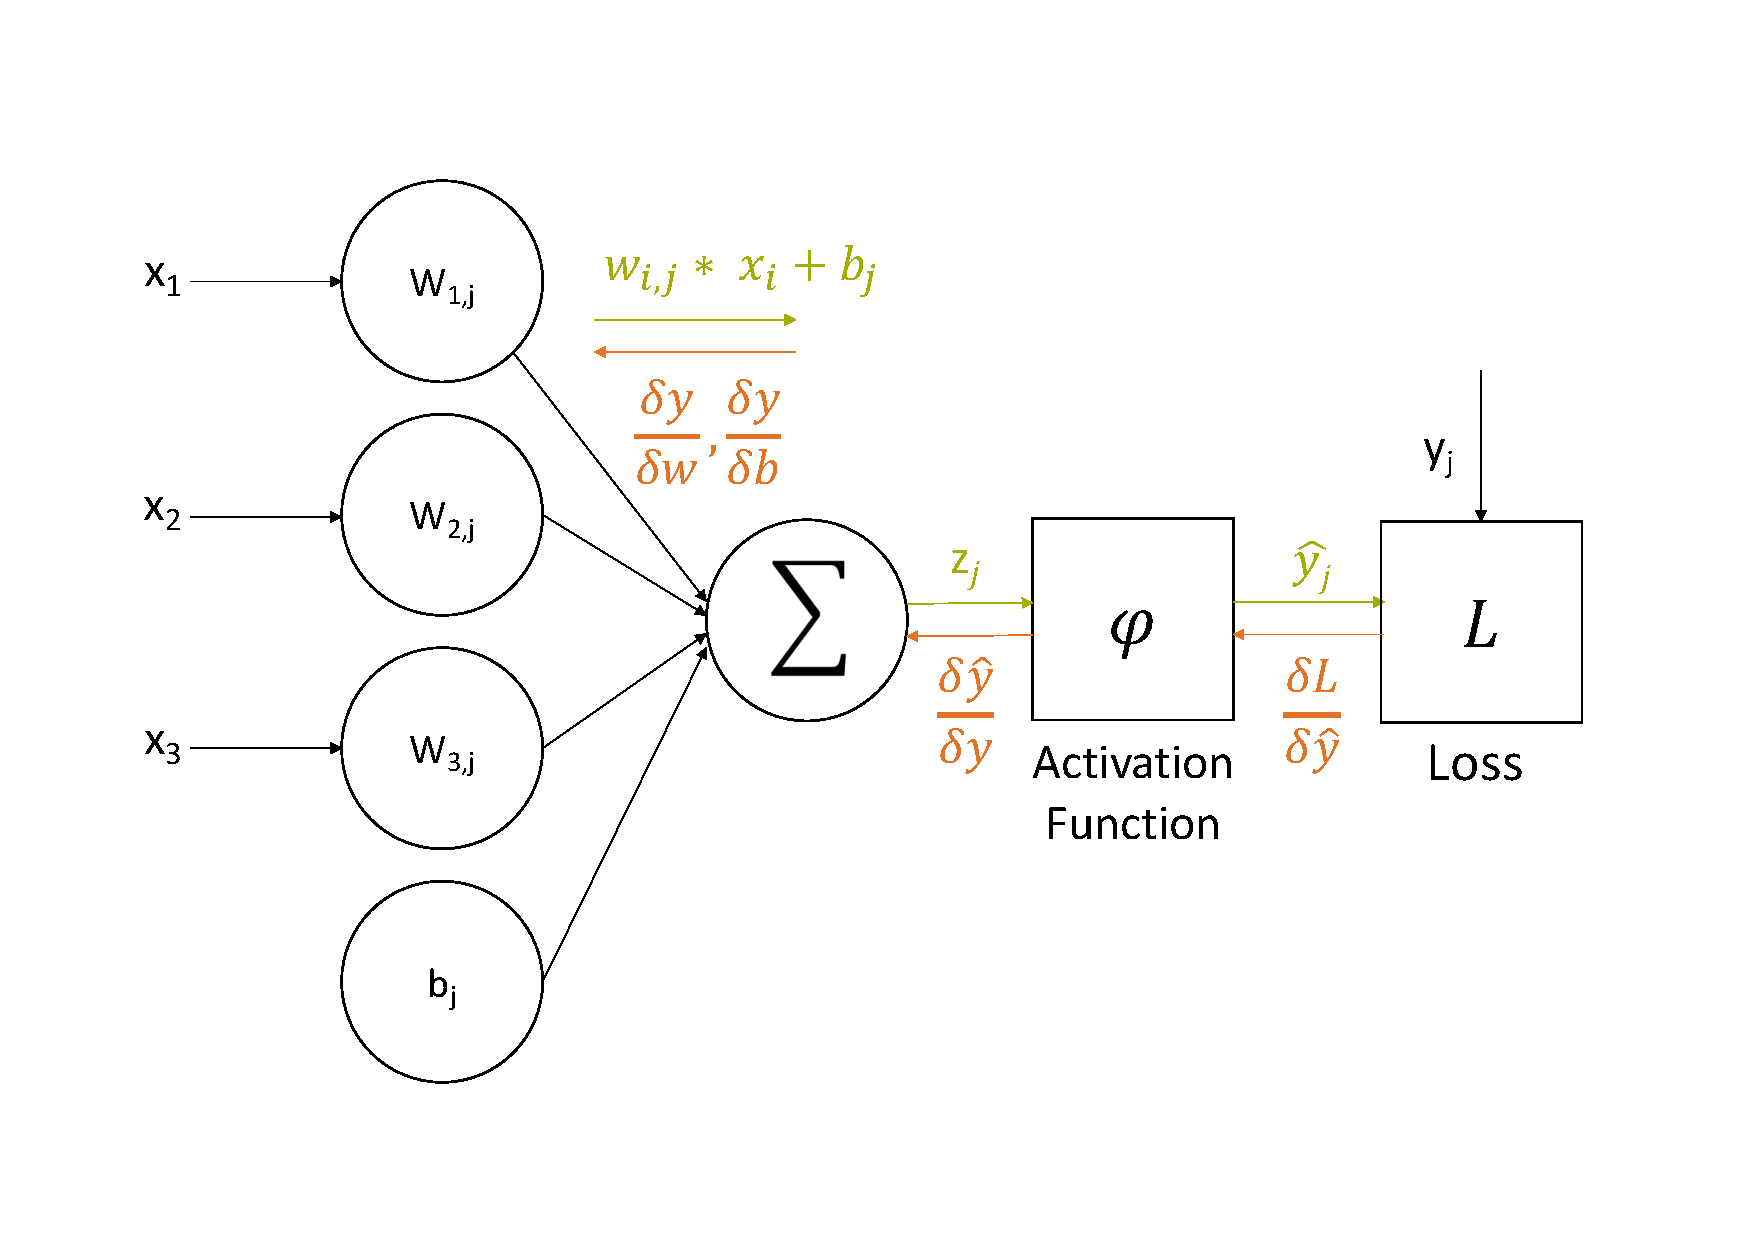
\includegraphics[width=0.7\textwidth]{neural_network_optimization.pdf}
  \caption {Optimization of neural network}
  \label{fig:neural_network_optimization}
\end{figure}

\section{Convolutional Neural Network}

Equally, to regular neural networks, convolutional neural networks (CNNs) consist of several neurons embedded in a fixed architecture. Developed for computer vision applications, the architecture of CNNs is optimized to process images. In CNNs the neurons are structured in layers just like in normal neural networks. In regular networks the neurons of a layer are organized in one dimension and in CNNs in three dimensions (height, width, depth) \cite{OShea2015}. The functionality of CNNs is visualized in \ref{fig:CNN_overview}. One can identify four main compounds of a CNN, which are described more detailed in the following:

\begin{itemize}
    \item [1.] The input data is organized in a structured and grid-like form. Each element in this structure is called a pixel, which is specified by a value and position. In the latent feature spaces, the data is stored as arrays with spatial dimension (height x width) and depth (channel size) \cite{OShea2015}.
    
    \item [2.] Convolutional layers contain kernels which are convolved with the input. The kernel contains weights and biases, which are learned during training. An elementwise activation function is applied to the kernel outputs \cite{OShea2015}.
    
    \item [3.]  Pooling layers downsample the spatial dimension. This reduces the height and width of the feature maps throughout the network. The learnable network parameters are minimized \cite{OShea2015}.
    
    \item [4.] Final fully-connected layers coupled with activation functions predict class labels for the input data \cite{OShea2015}.
\end{itemize}

\begin{figure}[H]
  \centering
  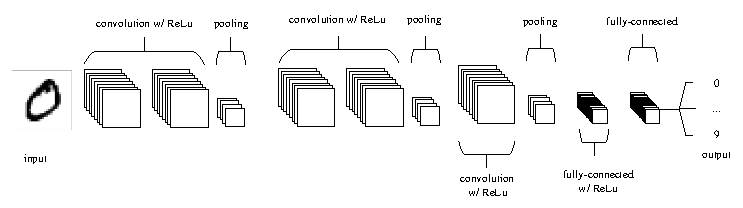
\includegraphics[width=0.9\textwidth]{cnn/cnn_architecture.pdf}
  \caption {CNN architecture \cite{OShea2015}}
  \label{fig:CNN_overview}
\end{figure}

In the following typical CNN layers are described more in detail. 

\subsection{Convolutional Layer}
The convolutional layers are the core elements in CNNs. The learnable parameters in a convolutional layer are the weights and biases of the corresponding kernel. During the optimization, each kernel learns to extract expressive features. The depth of a kernel is defined by the depth of the input layer and the number of applied kernels defines the depth of the subsequent feature map. Usually, the spatial dimensions (width, height) are reduced and the depth of the latent feature map is increased throughout the network. Therefore, the network extracts more global features in the beginning and more local features in the end of the network \cite{OShea2015}. Looking at fig. \ref{fig:kernel_number} one can see how the kernel of depth 3 is applied to the input of depth 3. By using 6 kernels, the resulting feature map is of depth 6.

\begin{figure}[H]
  \centering
  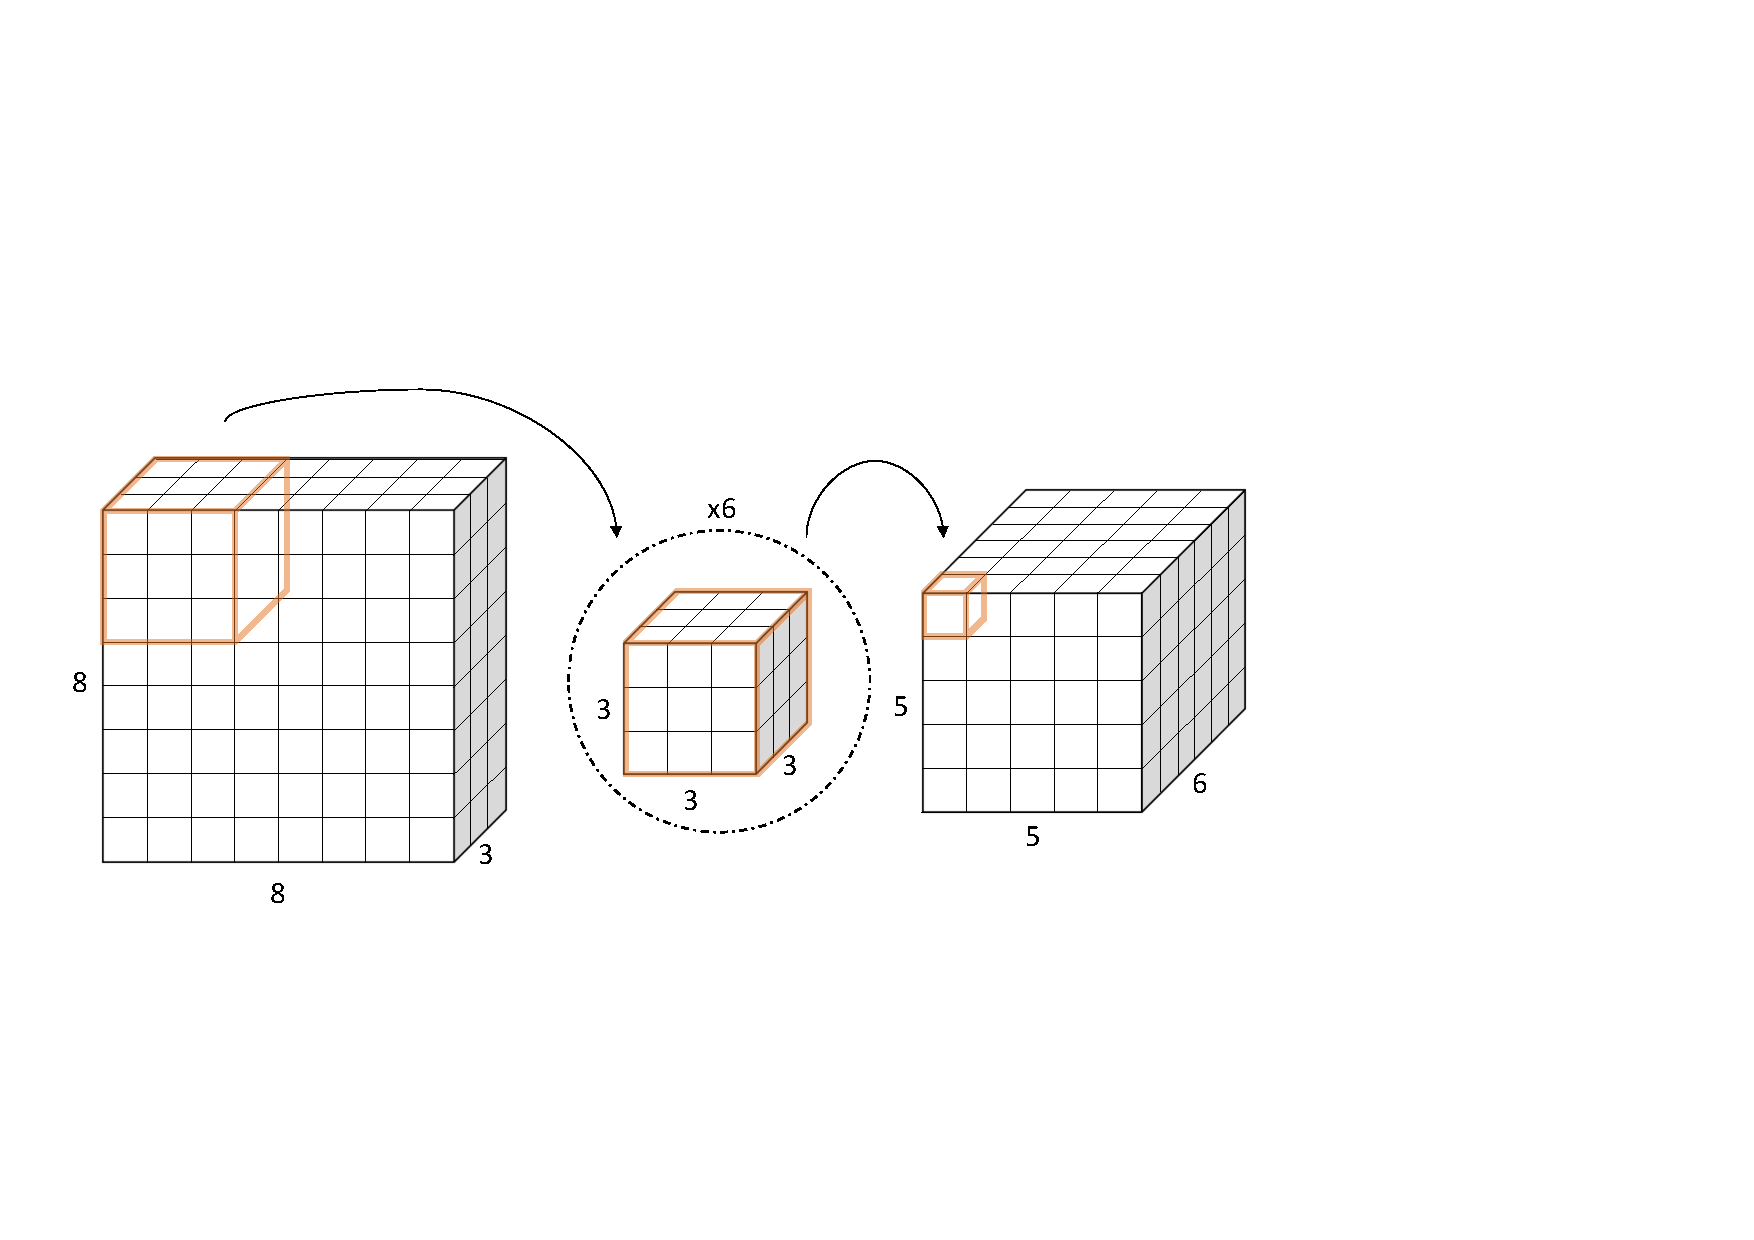
\includegraphics[width=0.8\textwidth]{cnn/kernel_number.pdf}
  \caption {2D convolution}
  \label{fig:kernel_number}
\end{figure}

To make things easier, the convolution of a kernel with an input subspace is shown for the 1D case:

\begin{equation}
  y(p_{0}) = \sum_{p_{n} \in R} w(p_{n}) \cdot x(p_{0} + p_{n}), 
  \label{eq:kernel}
\end{equation}

where $p_{n}$ is one of the $R$ kernel cells, $p_{0}$ is the lower bound pixel position of the input subspace involved in the convolutional operation. Each kernel cell is multiplied with a corresponding input pixel. The $R$ outputs are summed up in the pixel $p_{0}$ of the subsequent feature map \cite{Dai2017}. Typically, a bias value is included in this weighted sum and a non-linearity is applied consecutively. The convolutional process is visualized in fig. \ref{fig:kernel}.


\begin{figure}[H]
  \centering
  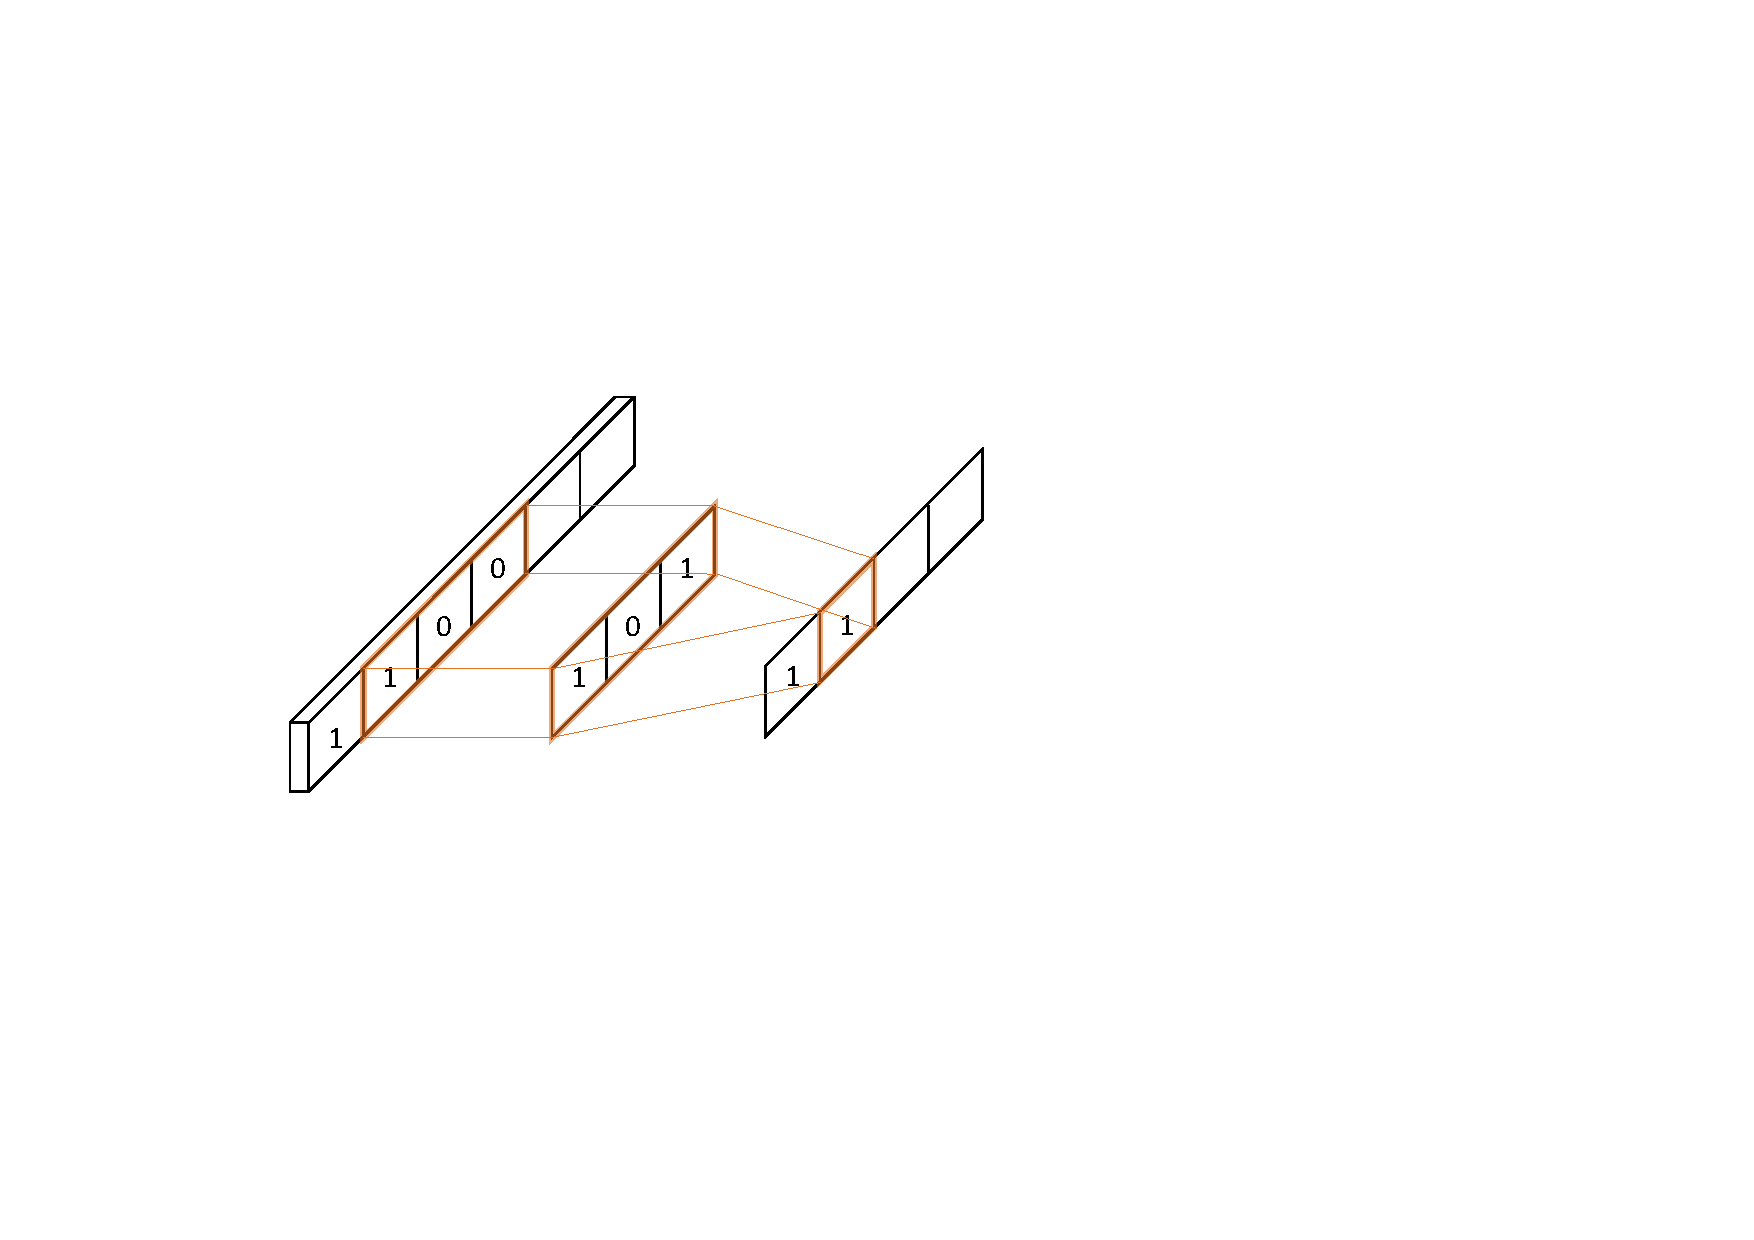
\includegraphics[width=0.4\textwidth]{cnn/kernel_calculation.pdf}
  \caption {1D convolution}
  \label{fig:kernel}
\end{figure}

Compared to regular neural networks CNNs profit a lot from its weight sharing concept. The kernel weights are learned throughout the training. Since the same kernel is applied on different areas of the input, it is not necessary to train a weight for every input pixel. This reduces the number of learnable parameters in the network. Since the kernel is applied on different input subsapces, the feature search is insensitive to the feature location in the image \cite{OShea2015}.

\subsection{Convolution Parameters}
When defining a CNN architecture, one has to find a trade-off between training effort and model complexity. The CNN should be able to capture relevant information from the data without requiring extensive optimization. The spatial dimension of the output of a convolutional operation ($V_{out}$) is defined by the stride ($S$), zero padding ($Z$), the receptive field ($R$) and the spatial dimension of the input ($V_{in}$): 
\begin{equation}
  V_{out} = \frac{(V_{in}-R)+2Z}{S+1}, 
  \label{eq:spatial_dimensionality_cnn_feature map}
\end{equation}

These parameters significantly influence the characteristic of CNNs, which is the reason why they are specified in more detail in the following.

\subsubsection{Stride}
The stride defines the number of pixels skipped while shifting the kernel over the input. By increasing the stride, the spatial dimension of the resulting feature map is decreased and otherwise increased \cite{OShea2015}. Fig. \ref{fig:stride_cnn} visualizes the effect of the stride on the convolutional operation.

\begin{figure}[H]
  \centering
  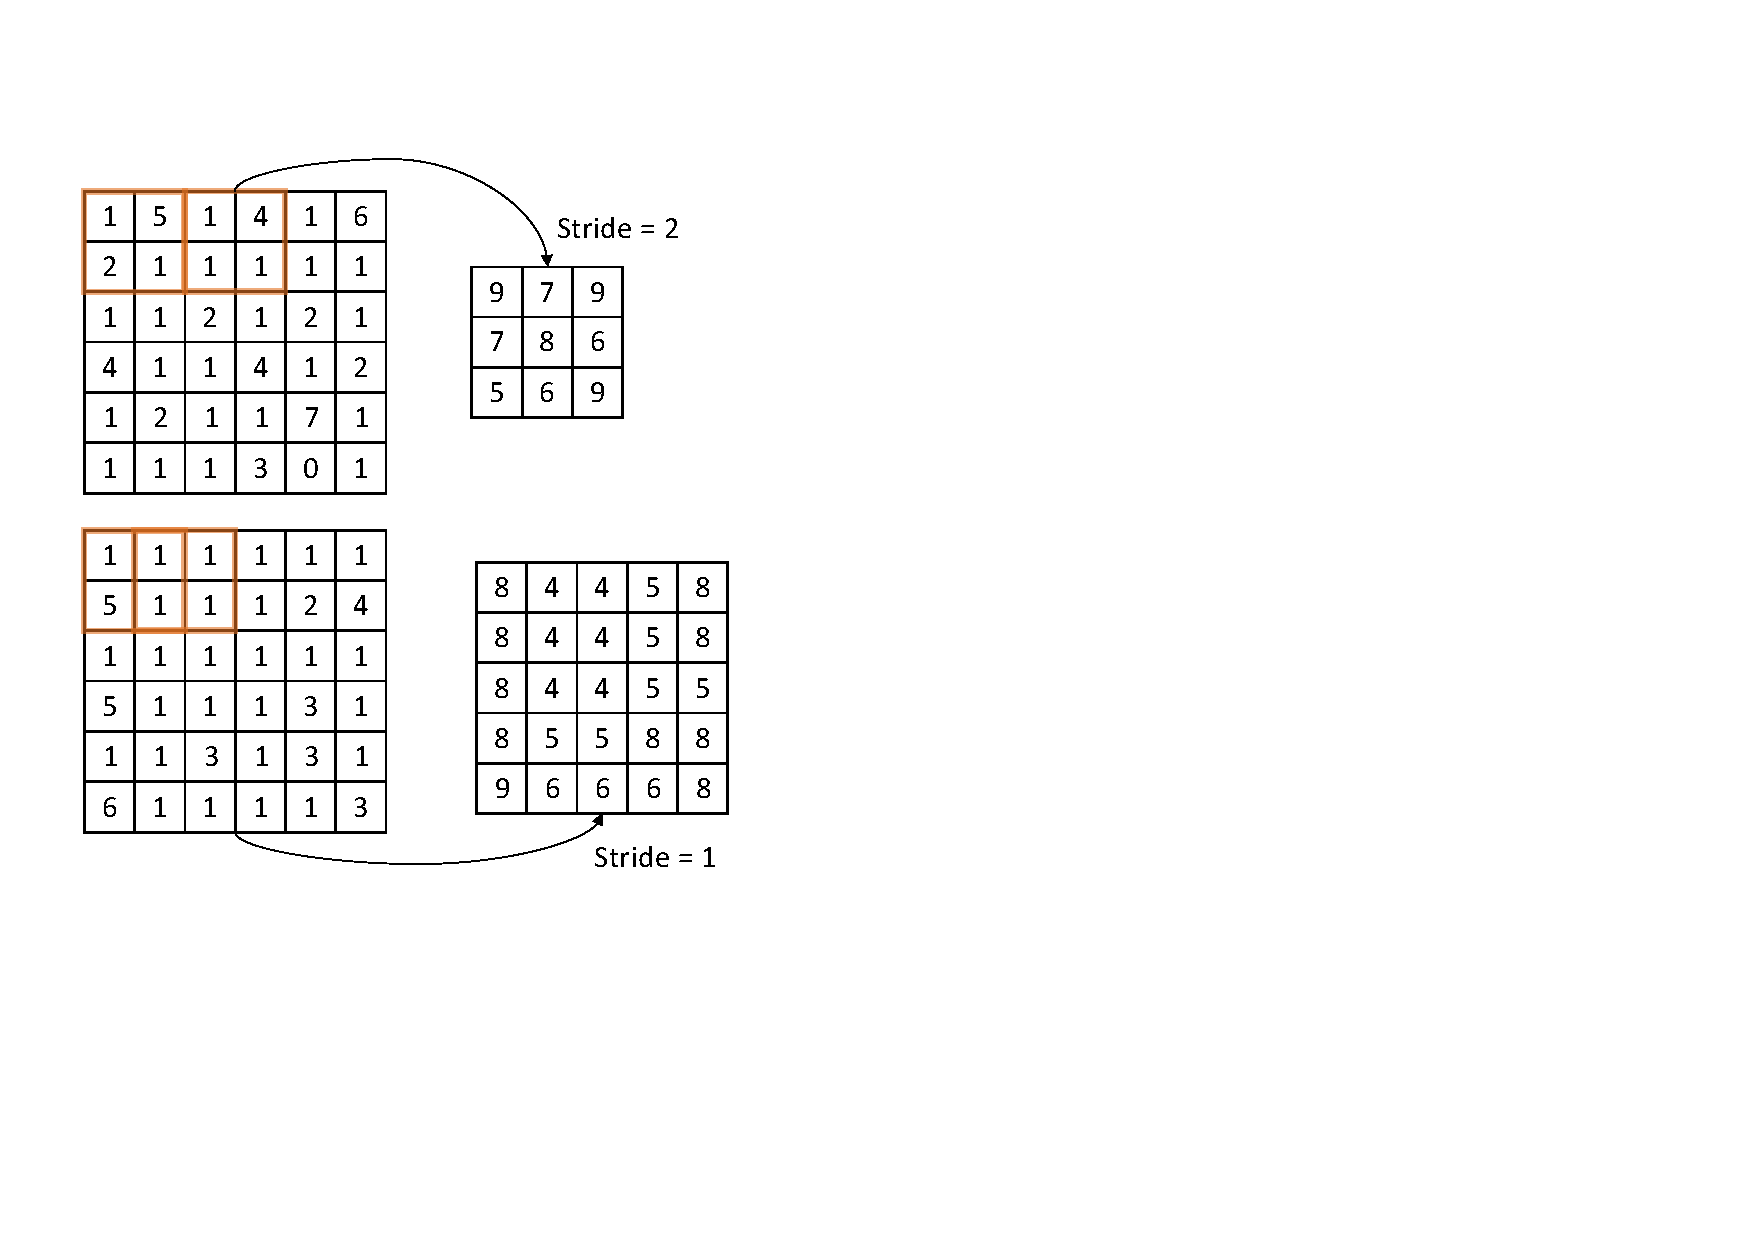
\includegraphics[width=0.45\textwidth]{cnn/stride_cnn.pdf}
  \caption {Stride factor}
  \label{fig:stride_cnn}
\end{figure}


\subsubsection{Zero Padding}
Zero padding, shown in fig.\ref{fig:zero_padding_cnn}, enlarges the input with a border of zeros. During the convolution, the kernel covers an increased spatial dimension, which increases the spatial dimension of the resulting feature map \cite{OShea2015}.

\begin{figure}[H]
  \centering
  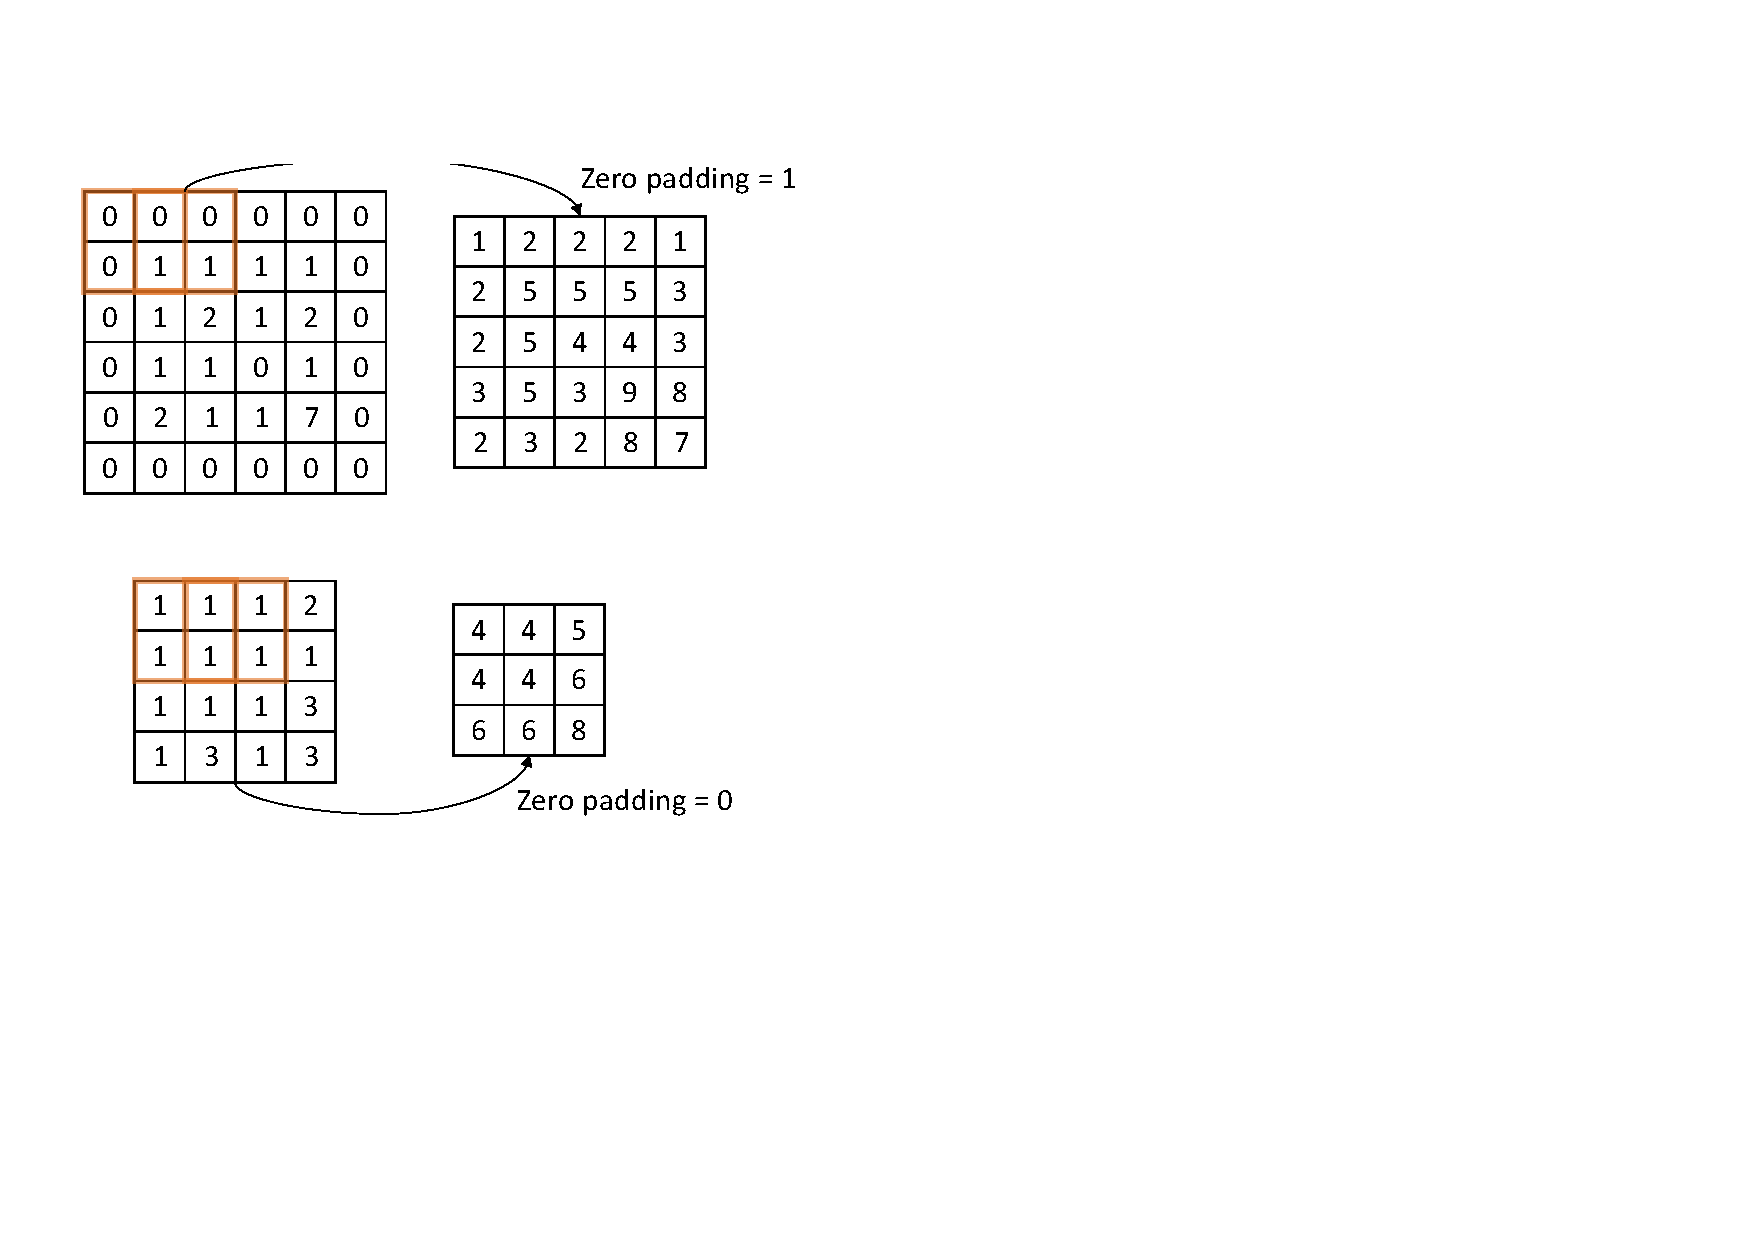
\includegraphics[width=0.5\textwidth]{cnn/zero_padding_cnn.pdf}
  \caption {Zero padding}
  \label{fig:zero_padding_cnn}
\end{figure}

\subsubsection{Receptive field}
The spatial dimension of the input subspace, which is covered by the kernel during a single convolution, is called receptive field. When increasing the receptive field, more global and otherwise more local features of the input are extracted. The receptive field is defined by the spatial dimension of the kernel \cite{OShea2015}. Dilated convolution can be applied to increase the receptive field size while maintaining the model complexity \cite{Dai2017}. 

\subsection{Pooling Layer}
Pooling layers are applied to change the spatial dimension of the latent feature spaces throughout the network. In general, the functionality is similar to convolutional layers with the only difference that no learnable parameters are involved. Pooling kernels are shifted over the input just as regular kernels in convolutional layers. For each kernel position, all pixels covered by the kernel are merged in a single value. Max-pooling layers return the maximal and AVG-pooling layers the average pixel value from all pixels covered by the kernel. The differences between Max-pooling and AVG-pooling layers is shown in fig. \ref{fig:Pooling_types}. Often convolutional and pooling layers are applied consecutively \cite{OShea2015}.

\begin{figure}[H]
  \centering
  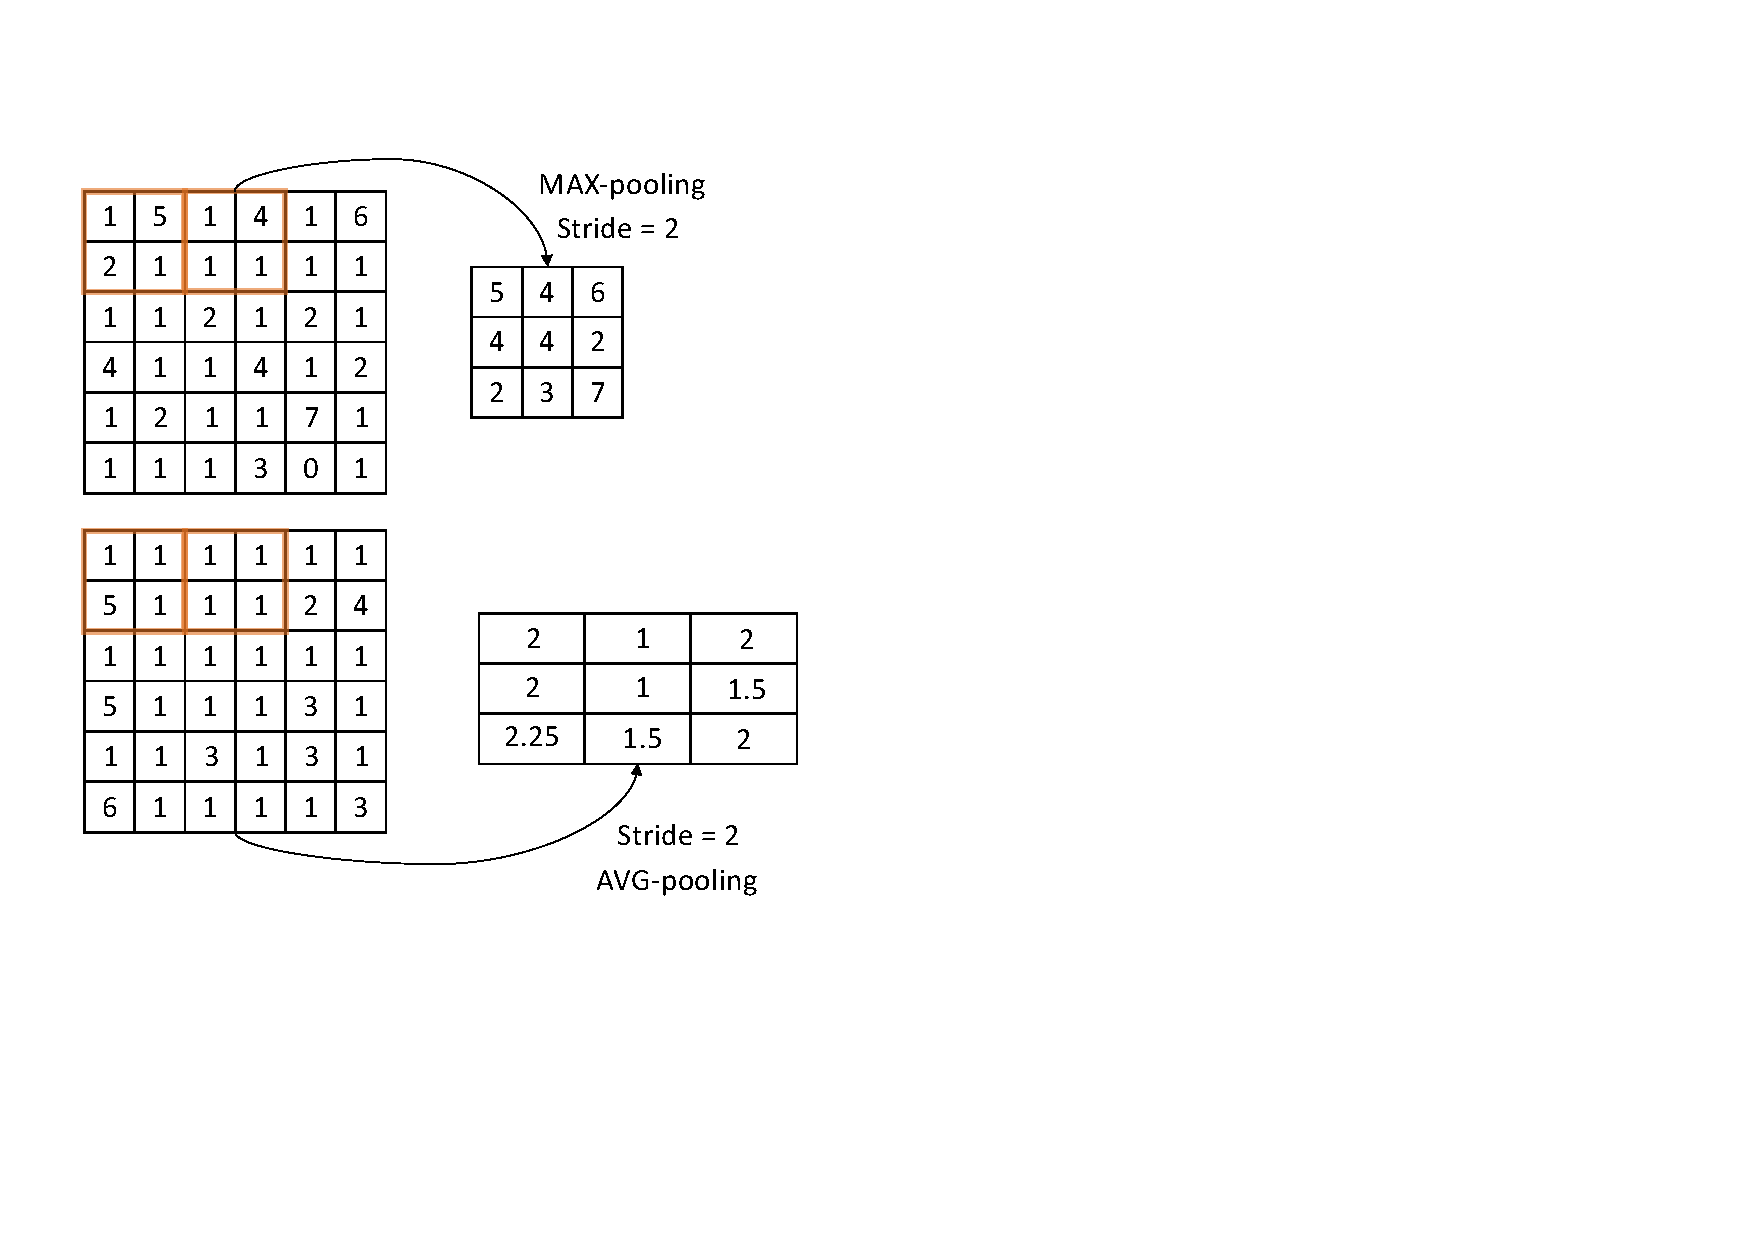
\includegraphics[width=0.5\textwidth]{cnn/Pooling_types.pdf}
  \caption {Pooling types}
  \label{fig:Pooling_types}
\end{figure}

\section{Domain Adaptation and Transfer Learning}

In the computer vision community, domain adaptation and transfer-learning techniques recently received more and more attention. Transfer learning addresses applications, in which a model is trained to solve a specific task on a given dataset. The model is then applied to solve a different task on that same dataset. The marginal data distribution is equal but the conditional distribution does change for both tasks. Domain adaptation solves problems, in which a model is trained on a labeled train dataset, denoted as source domain. The model is then applied to solve the same task on a different unlabeled test dataset, denoted as target domain. The data distribution of the target and source domain is different but the data must be related in any sense and structured similarly. The conditional and marginal distribution differ for both tasks. The differences are visualized in fig. \ref{fig:domain_adaption_vs_transfer_learning}

\begin{figure}[H]
  \centering
  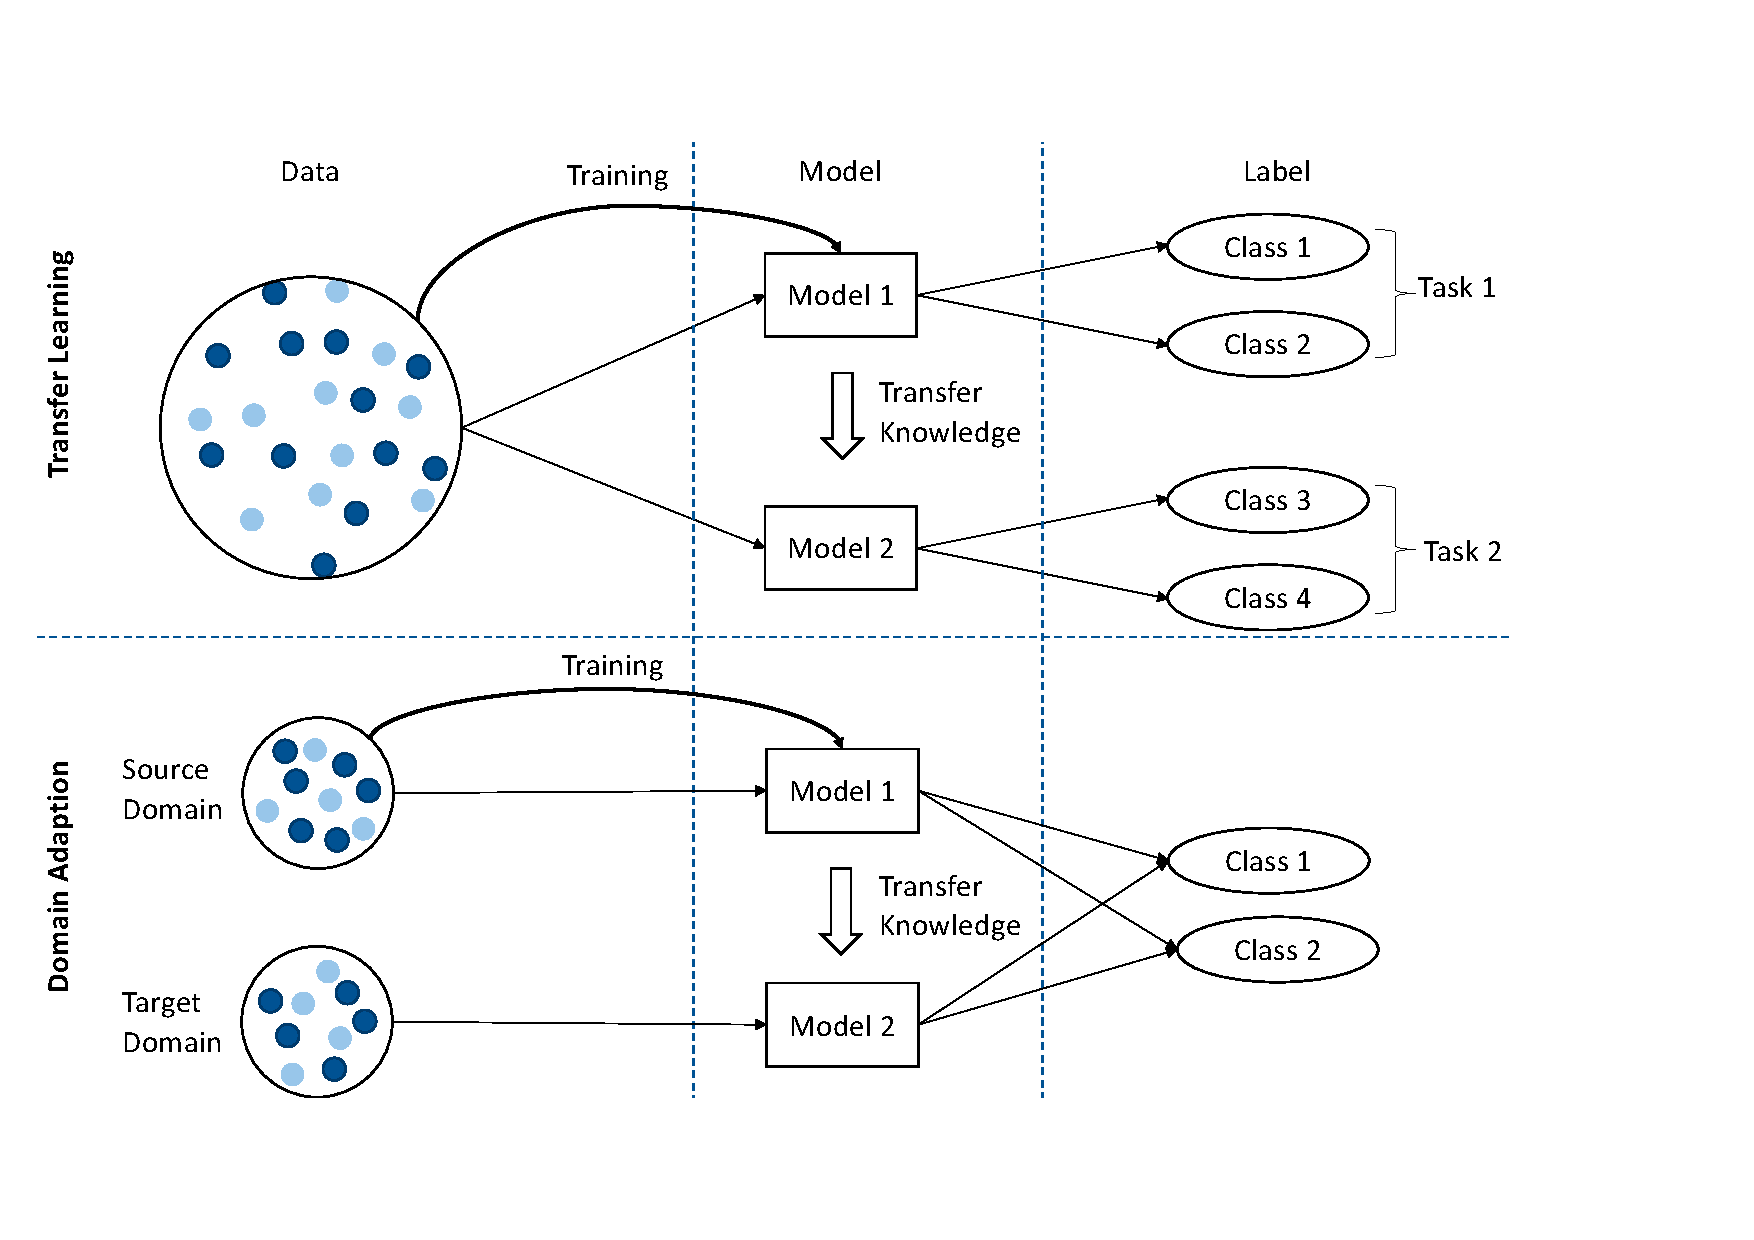
\includegraphics[width=.8\textwidth]{domain_adaption_vs_transfer_learning.pdf}
  \caption {Transfer learning vs. domain adaptation} \label{fig:domain_adaption_vs_transfer_learning}
\end{figure}


Since the focus of this thesis is to analyze domain adaptation approaches, the following passages explain the different aspects of domain adaptation.
\subsection{Notation}
The labeled source domain data is denoted by  $S = {(x_{i}^{s}, y_{i}^{s})_{i = 0}^{i = N_{s}}}$. Generally, the target domain data is separated in labeled $T_{l} = {(x_{i}^{tl}, y_{i}^{tl})_{i = 0}^{i = N_{tl}}}$ and unlabeled data $T_{u} = {(x_{i}^{tu})_{i = 0}^{i = N_{tu}}}$. It is assumed that there is a large amount of labeled data in the source and in some cases a small amount of labeled data in the target domain available ($N_{tl} \ll N_{s}$). The input samples are defined by $x_{i}$ and the corresponding label $y_{i}$  \cite{Patel2015}. Depending on the data available during training, one differs between different domain adaptation methods: 
\begin{itemize}
\item \textbf{Semi-supervised domain adaptation}, where a function is trained to use the data from $S$, $T_{l}$ \cite{Patel2015}. 
\item \textbf{Unsupervised domain adaptation}, where a function is learned using the data from $S$ and $T_{u}$ \cite{Patel2015}.
\end{itemize}

From a statistical point of view, the source and target domain can be described by the marginal distribution $P(X)$ and conditional distribution $P(Y|X)$. The data from source and target have the same data space and label space, but the marginal and conditional distribution differs $P(Y_{s}) \neq P(Y_{t})$ and $P(Y_{s}|X_{s}) \neq P(Y_{t}|X_{st})$ \cite{Qikang2020}

\subsection{Types of Domain Adaption}
Generally, domain adaptation approaches can be grouped in four different types:  

\begin{itemize}
\item \textbf{Instance Weighting Methods} address the covariate shift by integrating weights into a loss function, which estimate the similarity between source and target samples. Weighting factors like $\frac{P_{t}(x)}{P_{s}(x)}$ can be used. Source domain sample, which have a high probability to be in the target domain, are quite similar to the target domain samples. Samples like that should be strongly included in the training to optimize the model to work well on the target domain data \cite{AZAMFAR2020103932}.
\item \textbf{Feature-Based Methods} find a feature space which reduces the domain discrepancy. All source and target samples are transferred in the domain-invariant feature space, where the classification problem is identical for both domains \cite{AZAMFAR2020103932}. Fig. \ref{fig:Domain_adaption_intro} illustrates how feature-based domain adaptation can be used to find a cross-domain classifier, which accurately separates source and target domain data \cite{AZAMFAR2020103932}. 
\item \textbf{Model-Based Methods} train a classifier on the source domain, which can be transferred or fine-tuned to perform well on the target domain \cite{AZAMFAR2020103932}.
\item \textbf{Relation-Based Methods} utilize similarities between the two domains in order to transfer knowledge between the domains\cite{AZAMFAR2020103932}. 
\end{itemize}

\begin{figure}[H]
  \centering
  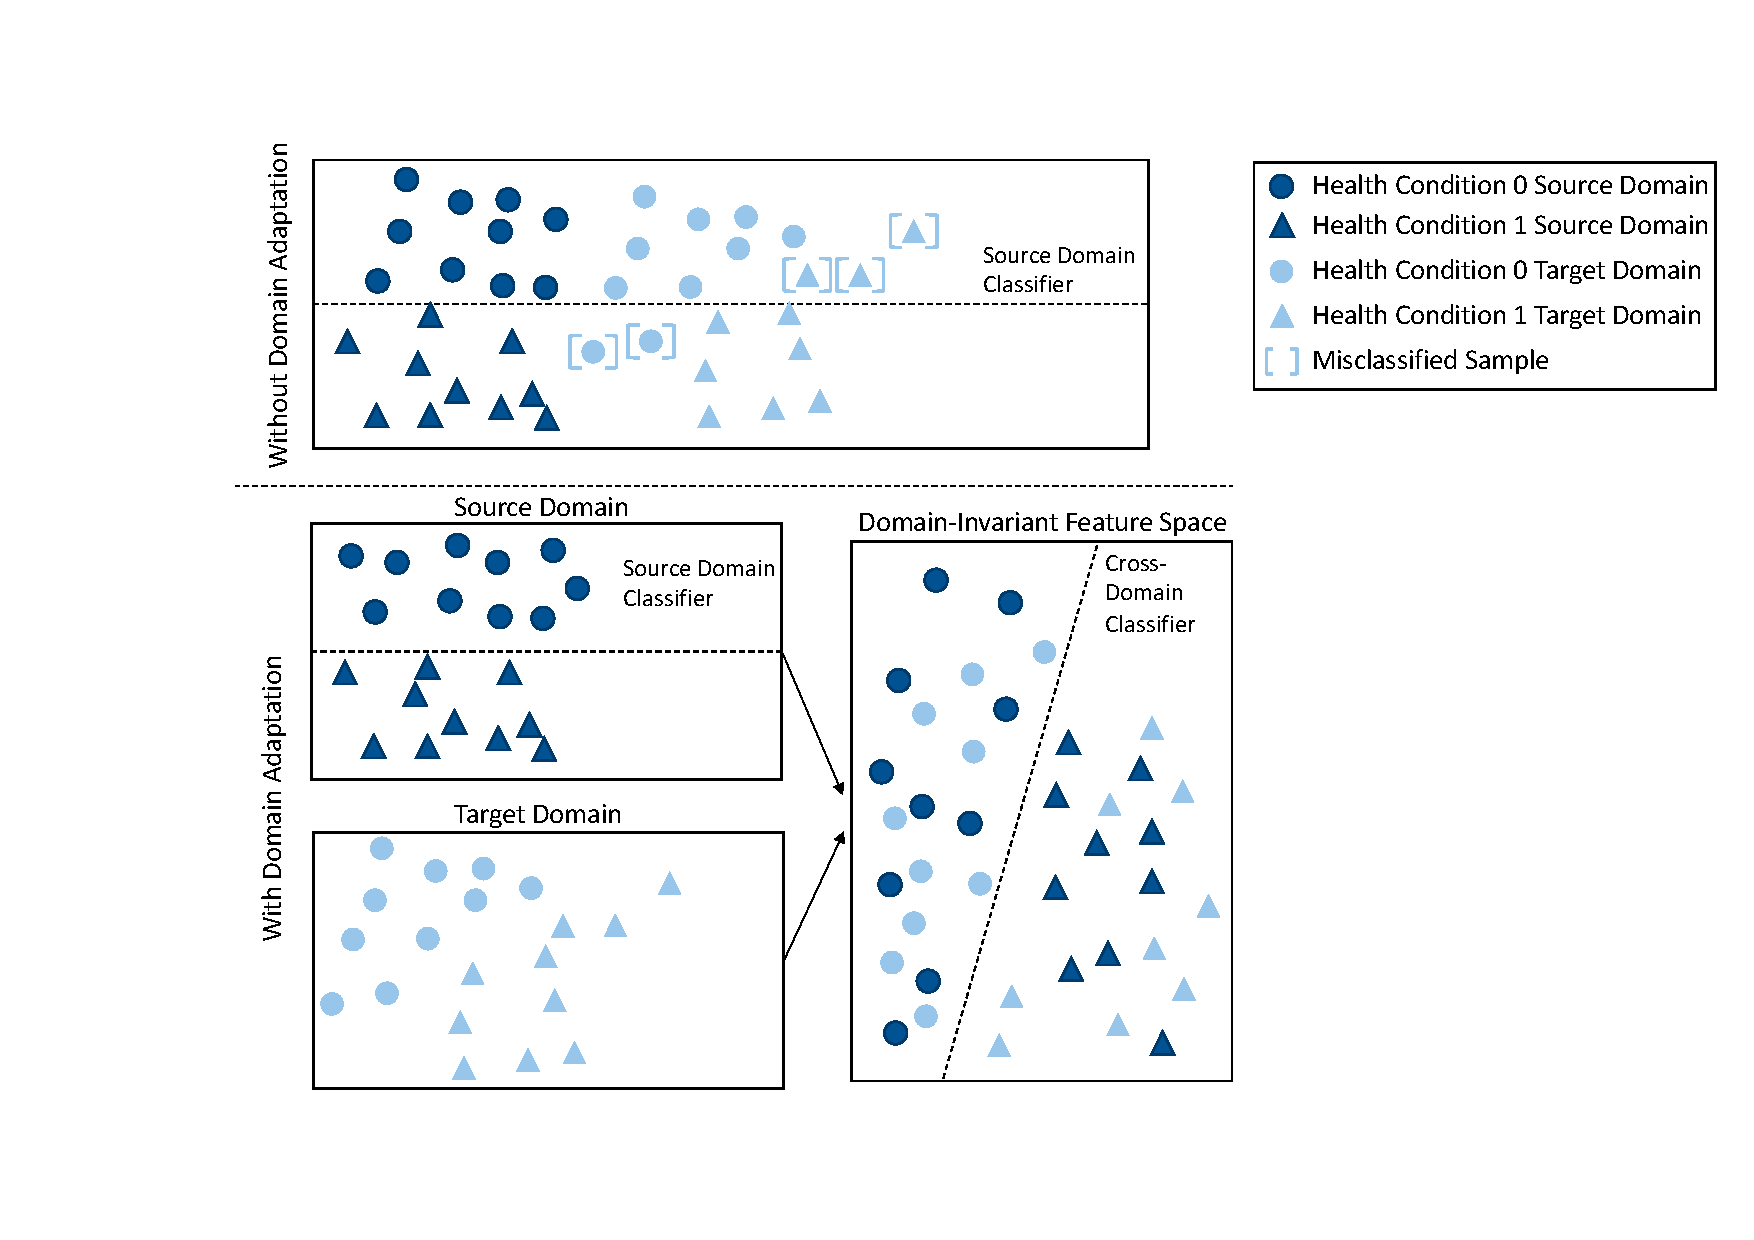
\includegraphics[width=1\textwidth]{domain_adaption_intro.pdf}
  \caption {Domain adaptation for PHM based on \cite{Pandhare2021}} \label{fig:Domain_adaption_intro}
\end{figure}


\section{Maximum Mean Discrepancy}
Maximum Mean Discrepancy (MMD) is a criterion which estimates the discrepancy between two distributions. MMD can be used to optimize a neural network such that the distribution discrepancy in its latent feature space is reduced. In the reproducing kernel Hilbert space (RKHS) the discrepancy is measured as squared distance between the distribution kernel embeddings. The distribution discrepancy across domains can be measured in several layers of the neural network. Including this information in the optimization of the model helps to avoid feature transferability degradation \cite{li2020}. The MMD criterion is defined as following:

\begin{align}
    M_{k}(P,Q) = \Bigl|  \boldsymbol{E_{P}}[\Phi(\boldsymbol{X^{s}})] - \boldsymbol{E_{Q}}[\Phi(\boldsymbol{X^{t}})]     \Bigl|^{2}_{Hk},
\end{align}

where Hk denotes the RKHS, which is described by the characteristic kernel k and the mapping function $\Phi$. When taking the identity function as mapping function, the discrepancy between the distribution means is measured. When using more complex mapping functions also higher order moments can be matched \cite{Yujia2015}. The distributions of the source domain $X^{s} = \{{x}_{i}^{s}\}_{i=0,...,n_{s}}$ and target domain $X^{t} = \{{x}_{i}^{t}\}_{i=0,...,n_{t}}$ in the latent feature space of interest are represented by $P$ and $Q$ and the corresponding expectations by $\boldsymbol{E_{P}[\cdot]}$ and $\boldsymbol{E_{Q}[\cdot]}$. The kernel choice is of great importance when applying MMD for optimizing neural networks. For this reason, it makes sense to combine several kernels to profit from their individual performance:

\begin{align}
    k(\boldsymbol{X^{s}}, \boldsymbol{X^{t}}) = \sum_{i=0}^{N_{k}} k_{\sigma_{i}}(\boldsymbol{X^{s}}, \boldsymbol{X^{t}}),
\end{align}

where $N_{k}$ denotes the number of kernels used in the RKHS and $k_{\sigma_{i}}$ represents one individual RBF kernels  \cite{li2020}. Other kernels like linear kernels could be used, but current research shows that RBF kernels usually perform best \cite{AZAMFAR2020103932}.


\section{Non-Stationary Signal Analysis for Prognostic and Health Management}
Non-stationary signal analysis, which is a method to investigate signals with changing statistical properties, is one of the main topics in the field of machinery fault diagnosis. Signals can contain multiple frequencies and amplitudes which might change over time. Traditional signal analysis techniques make stationary assumptions. When applying those to non-stationary signals, solely statistical averages in time or frequency can be extracted \cite{FENG2013}. Therefore, the demand for analysis methods, which allow to ascertain features of non-stationary signals, is increasing. Such methods seem promising for extracting health related information from machine data. Time–frequency representations (TFRs) are techniques to transform non-stationary signals in a two-dimensional time-frequency planes, where each value describes the dominance of a specific frequency at a certain point in time. All TFRs, which fulfill the idea of linearity and superposition, are called linear TFRs. The two most popular linear TFRs are the short-time Fourier and the Wavelet transform \cite{Hlawatsch1992}. 


\subsubsection{Short-Time Fourier transform}
Short-time Fourier transform (STFT) is a method which adds a time variable to the traditional Fourier spectrum. This allows to investigate variations in the signal spectrum over time. STFT assumes the spectrum to be constant during a short time window. For each such window a Fourier spectrum is obtained. The time related changes are measured between consecutive window snapshots. The process is mathematically expressed in the following:  
\begin{equation}
    STFT_{x}(t,f) = \int_{- \inf}^{+ \inf}x(\tau) w(\tau -t) exp(-j2\pi f \tau),
\end{equation}
where  $w(\tau -t)$ is the window function centered around t, which is multiplied with the signal $x(t)$. Specific window functions are defined to separate the signal. Shifting the window over the signal and applying the Fourier transform $exp(-j2\pi f \tau)$ to each window, generates a local frequency spectrum of the signal for different points in time \cite{FENG2013}. The time-frequency resolution is defined by the windowing function and the window length. STFT suffers from a trade-off between high resolution in time or frequency. The optimum window length depends on the main interest behind the signal analysis. For accurate time domain information the window size needs to be reduced and for frequency domain information increased. STFT  decomposes the signal in existing sinusoidals and determines its frequency and phase for a local part of the signal \cite{Hlawatsch1992}. 

\subsubsection{Wavelet Transform}
The Wavelet transform decomposes the signals in several wavelets. A wavelet is a wave-like oscillation, which is described by its function, location and scale. The location defines where the wavelet overlaps with the signal and the scale defines how much squished (small scale) or stretched (big scale) the wavelet is \cite{Sifuzzaman2009}. The convolution of the wavelet and the signal is mathematically expressed as following:
\begin{equation}
    WT_{x}(t,a) = \frac{1}{\sqrt{a}} \int_{- \inf}^{+ \inf} x(\tau) \psi(\frac{\tau -t}{a}) d \tau,
\end{equation}
 where $x(t)$ is the signal, $\psi(\frac{\tau -t}{a})$ the wavelet, $a$ the scaling factor, $t$ the time shift and $\frac{1}{\sqrt{a}}$ a normalization factor to maintain the energy conservation \cite{FENG2013}. Different wavelet bases $\psi(t)$ can be convolved with the signal, which allows to analyze the signal for different patterns \cite{Sifuzzaman2009}. Popular wavelet bases are the Gaussian, Morlet, Shannon, Meyer, Laplace, Hermit, or the Mexican Hat wavelets in both simple and complex functions \cite{Verstraete2017}. This enables a more extensive, flexible and detailed analysis. The wavelet transform can be adapted to extract patterns, which are especially relevant for a PHM task. In fig. \ref{fig:ricker_wavelet}, Ricker wavelets with different scales and locations are visualized. Wavelet transforms can extract local spectral and temporal information in parallel \cite{Sifuzzaman2009}.


\begin{figure}[H]
  \centering
  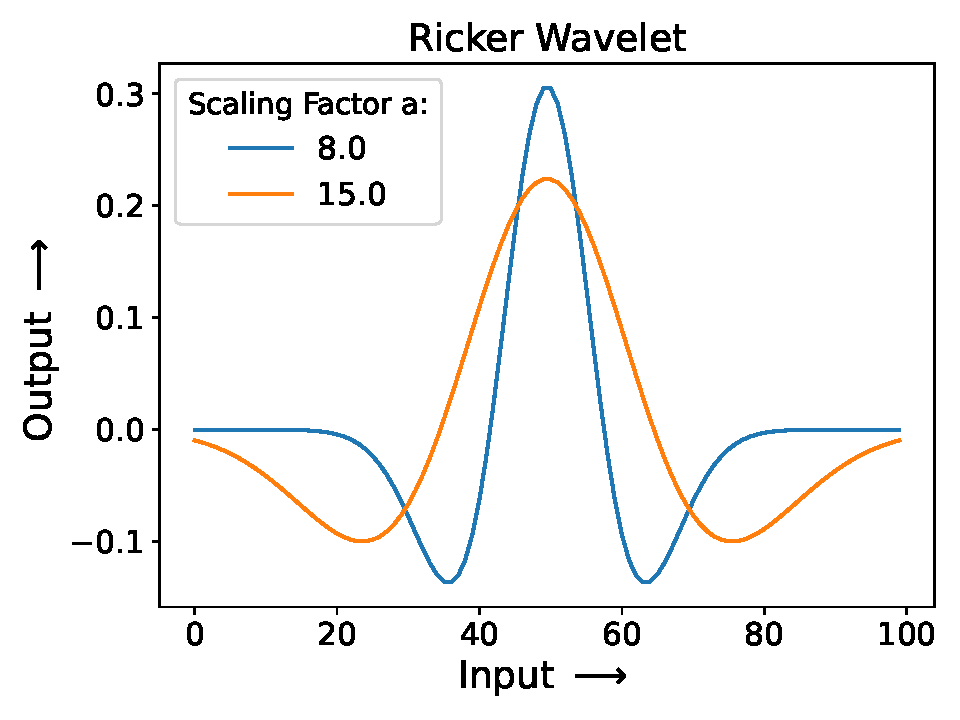
\includegraphics[width=.47\textwidth]{preprocessing_transform/Ricker_Wavelet_Scaling.pdf}
  \hspace{.1cm}
  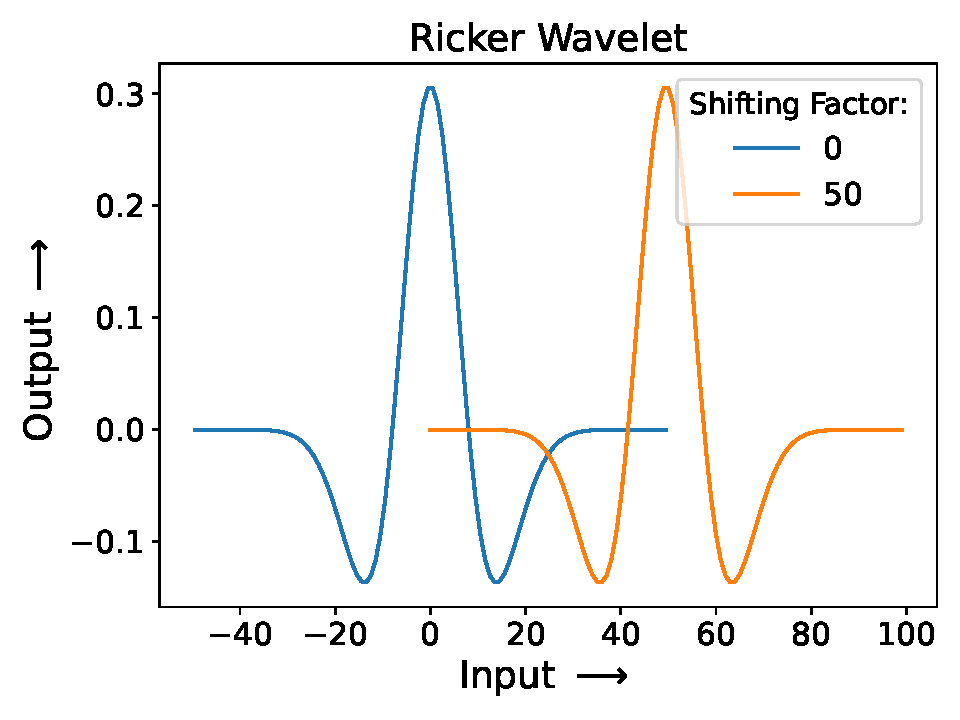
\includegraphics[width=.47\textwidth]{preprocessing_transform/Ricker_Wavelet_Shifting.pdf}
  

  \caption{Ricker wavelet}
  \label{fig:ricker_wavelet}
\end{figure}

\subsubsection{Spectrograms and Scalograms}

 Spectrograms are a graphic representation of the STFT and scalograms of the wavelet transform. Spectrograms and scalograms visualize the the squared magnitudes of the previously presented STFT and Wavelet transform. This squared magnitude is loosely interpreted as signal energy \cite{Hlawatsch1992}. The mathematical expressions are presented in the following: 

\begin{equation}
    \begin{aligned}
        SPEC_{x}(t,f) &= |STFT_{x}(t,f)|^{2} \\
        SCAL_{x}(t,f) &= |WT_{x}(t,f)|^{2}, 
    \end{aligned}
\end{equation}

where $STFT_{x}(t,f)$ is the Short-time Fourier transform, $WT_{x}(t,f)$ the wavelet transform, $SPEC_{x}(t,f)$ the spectrogram and $SCAL_{x}(t,f)$ the scalogram \cite{Hlawatsch1992}. This way of representing the system energy in the 2D time and frequency space may reveal useful information from a complex and high-dimensional signal without the need for additional feature extraction. As described before, spectrograms have a fixed frequency resolution that is defined by the windows size. Scalograms on the other hand have a frequency-dependent frequency resolution \cite{Verstraete2017}.

